\documentclass[a4paper,10pt]{jsarticle}
\usepackage{color}
\usepackage[dvipdfmx]{graphicx}
\usepackage{amsmath}

\author{sankaku}
\date{\today}
\title{otofu sample}

\usepackage{otf}
\begin{document}
\maketitle

\section{\UTF{901a}\UTF{5e38}\UTF{306f}\UTF{8868}\UTF{793a}\UTF{3067}\UTF{304d}\UTF{306a}\UTF{3044}\UTF{6587}\UTF{5b57}}
\label{通常は変換できない文字のセクション}

\UTF{9ad9}

\UTF{fa11}

\UTF{9592}

\UTF{7934}

\UTF{6422}

\UTF{5a6d}

\UTF{9dd7}

\UTF{2460}\UTF{2461}\UTF{2462}\UTF{2463}\UTF{2464}\UTF{2465}\UTF{2466}\UTF{2467}\UTF{2468}\UTF{2469}

\UTF{2160}\UTF{2161}\UTF{2162}\UTF{2163}\UTF{2164}\UTF{2165}\UTF{2166}\UTF{2167}\UTF{2168}\UTF{2169}

\section{\UTF{30b3}\UTF{30e1}\UTF{30f3}\UTF{30c8}\UTF{306e}\UTF{30bb}\UTF{30af}\UTF{30b7}\UTF{30e7}\UTF{30f3}}
\label{コメントのセクション}





\% \UTF{3053}\UTF{3053}\UTF{306f}\UTF{30b3}\UTF{30e1}\UTF{30f3}\UTF{30c8}\UTF{3067}\UTF{306f}\UTF{3042}\UTF{308a}\UTF{307e}\UTF{305b}\UTF{3093}\UTF{3002}



\section{include\UTF{306a}\UTF{3069}}
\label{includeなどのセクション}

main.tex\UTF{304b}\UTF{3089}sub1.tex\UTF{3092}include\UTF{3057}\UTF{307e}\UTF{3059}\UTF{3002}

\UTF{3053}\UTF{308c}\UTF{306f}main.tex\UTF{3067}\UTF{53c2}\UTF{7167}\UTF{3055}\UTF{308c}\UTF{3066}\UTF{3044}\UTF{308b}\UTF{30d5}\UTF{30a1}\UTF{30a4}\UTF{30eb}sub1.tex\UTF{3067}\UTF{3059}\UTF{3002}

\UTF{9ad9}

\UTF{fa11}

\UTF{9592}

\UTF{7934}

\UTF{6422}

\UTF{5a6d}

\UTF{9dd7}

\UTF{2460}\UTF{2461}\UTF{2462}\UTF{2463}\UTF{2464}\UTF{2465}\UTF{2466}\UTF{2467}\UTF{2468}\UTF{2469}

\UTF{2160}\UTF{2161}\UTF{2162}\UTF{2163}\UTF{2164}\UTF{2165}\UTF{2166}\UTF{2167}\UTF{2168}\UTF{2169}

sub1.tex\UTF{3053}\UTF{3053}\UTF{307e}\UTF{3067}\UTF{3002}


main.tex\UTF{304b}\UTF{3089}sub2.tex\UTF{3092}input\UTF{3057}\UTF{307e}\UTF{3059}\UTF{3002}

\UTF{3053}\UTF{308c}\UTF{306f}main.tex\UTF{3067}\UTF{53c2}\UTF{7167}\UTF{3055}\UTF{308c}\UTF{3066}\UTF{3044}\UTF{308b}\UTF{30d5}\UTF{30a1}\UTF{30a4}\UTF{30eb}sub2.tex\UTF{3067}\UTF{3059}\UTF{3002}

\subsection{\UTF{901a}\UTF{5e38}\UTF{306f}\UTF{8868}\UTF{793a}\UTF{3067}\UTF{304d}\UTF{306a}\UTF{3044}\UTF{6587}\UTF{5b57} subsub1}
\label{通常は変換できない文字のセクション subsub1}
dir/subsub1.tex\UTF{3092}input\UTF{3057}\UTF{307e}\UTF{3059}\UTF{3002}

\UTF{3053}\UTF{308c}\UTF{306f}sub2.tex\UTF{3067}\UTF{53c2}\UTF{7167}\UTF{3055}\UTF{308c}\UTF{3066}\UTF{3044}\UTF{308b}\UTF{30d5}\UTF{30a1}\UTF{30a4}\UTF{30eb}dir/subsub1.tex\UTF{3067}\UTF{3059}\UTF{3002}

\UTF{9ad9}

\UTF{fa11}

\UTF{9592}

\UTF{7934}

\UTF{6422}

\UTF{5a6d}

\UTF{9dd7}

\UTF{2460}\UTF{2461}\UTF{2462}\UTF{2463}\UTF{2464}\UTF{2465}\UTF{2466}\UTF{2467}\UTF{2468}\UTF{2469}

\UTF{2160}\UTF{2161}\UTF{2162}\UTF{2163}\UTF{2164}\UTF{2165}\UTF{2166}\UTF{2167}\UTF{2168}\UTF{2169}

dir/subsub1.tex\UTF{3053}\UTF{3053}\UTF{307e}\UTF{3067}\UTF{3002}


sub2.tex\UTF{3053}\UTF{3053}\UTF{307e}\UTF{3067}\UTF{3002}


\section{includegraphics\UTF{306a}\UTF{3069}}
\label{includegraphicsなどのセクション}


main.tex\UTF{304b}\UTF{3089}dir/graph.tex\UTF{3092}input\UTF{3057}\UTF{307e}\UTF{3059}\UTF{3002}

\UTF{3053}\UTF{308c}\UTF{306f}main.tex\UTF{3067}\UTF{53c2}\UTF{7167}\UTF{3055}\UTF{308c}\UTF{3066}\UTF{3044}\UTF{308b}\UTF{30d5}\UTF{30a1}\UTF{30a4}\UTF{30eb}dir/graph.tex\UTF{3067}\UTF{3059}\UTF{3002}


\UTF{753b}\UTF{50cf}\UTF{30b5}\UTF{30f3}\UTF{30d7}\UTF{30eb}: \includegraphics[width=1cm]{img/not/converted.eps}

\UTF{3053}\UTF{308c}\UTF{306f}\UTF{30b3}\UTF{30de}\UTF{30f3}\UTF{30c9}\UTF{3067}\UTF{306f}\UTF{306a}\UTF{3044}: \\includegraphics[width=1cm]{img/not/converted.eps}

\UTF{30b3}\UTF{30de}\UTF{30f3}\UTF{30c9}\UTF{90e8}\UTF{3060}\UTF{3051}\UTF{5909}\UTF{63db}\UTF{3055}\UTF{308c}\UTF{308b} \\includegraphics[width=1cm]{\includegraphics[width=1cm]{img/not/converted.eps}}




\UTF{3053}\UTF{308c}\UTF{306f}\UTF{30b3}\UTF{30de}\UTF{30f3}\UTF{30c9}\UTF{3067}\UTF{306f}\UTF{306a}\UTF{3044}: \\includegraphics[width=1cm]{img/\UTF{3053}\UTF{3053}\UTF{306f}/\UTF{5909}\UTF{63db}/\UTF{3055}\UTF{308c}\UTF{308b}.eps}



dir/graph.tex\UTF{3053}\UTF{3053}\UTF{307e}\UTF{3067}\UTF{3002}



\section{ref\UTF{306e}\UTF{30bb}\UTF{30af}\UTF{30b7}\UTF{30e7}\UTF{30f3}}
\label{refのセクション}

\ref{通常は変換できない文字のセクション}\UTF{3001}\ref{includeなどのセクション}\UTF{3001}\ref{includegraphicsなどのセクション}\UTF{3001}\ref{refのセクション}\UTF{3092}\UTF{53c2}\UTF{7167}\UTF{306e}\UTF{3053}\UTF{3068}\UTF{3002}

\end{document}

